\chapter{طراحی معماری}

\section{فرایند طراحی معماری}	
طراحی معماری یک سیستم نرم‌افزاری یک فرایند شناختی تصمیم‌گیری به منظور تبیین ساختار کلی سیستم، زیرسیستم‌ها و ارتباط میان آنهاست و عوامل متعددی در این امر دخیل‌اند. از این عوامل می‌توان به نوع سیستم تحت توسعه و اهداف دنبال شده جهت طراحی معماری سیستم اشاره کرد. با توجه به اینکه طراحی معماری یک فرایند بازگشتی‌ست، هر سیستم متشکل از تعدادی زیرسیستم است و هر کدام از این زیرسیستم‌ها نیز از سطوح پایین‌تری تشکیل شده‌اند و تکرار فرایند بازگشتی طراحی برای هر سطح و تا پایین‌ترین سطح لازم است. پایان فرایند به عوامل گوناگونی نظیر اندازه و پیچیدگی سیستم، تجربه‌ی تیم توسعه و اهداف طراحی بستگی دارد.

\subsection{تبیین اهداف طراحی}			
ابتدا نیاز است که ملزومات اساسی و محدودیت‌های سیستم بنا بر شاخص‌های قابل توجه بررسی شوند:
\begin{enumerate}
	\item
	سادگی تغییر و نگهداری
	\item
	کاربرد قطعات تجاری
	\item
	کارایی سیستم
	\item
	قابلیت اطمینان
	\item
	امنیت
	\item
	حمل‌پذیری خطا
	\item
	ترمیم
\end{enumerate}

\subsection{تعیین نوع سیستم}
نوع یک سیستم، مدل‌سازی، تحلیل، طراحی، پیاده‌سازی و آزمون سیستم را بشدت تحت‌تاثیر خود قرار می‌دهد. به همین دلیل در زمان طراحی معماری نرم‌افزار، انتخاب نوع سیستم از اهمیت بالایی برخوردار است. با توجه به اهمیت تعامل بین سیستم و کنشگر برای انجام یک فرایند در \textit{کارتاپ} و اهداف طراحی معماری ذکر شده و همچنین موارد زیر، \textit{کارتاپ} یک سیستم تعاملی‌ست، معماری نرم‌افزاری \lr{N-Tire} برای آن انتخاب شده است.


\begin{enumerate}
	\item		
	تعامل بین سیستم و کنشگر برای انجام یک فرایند در \textit{کارتاپ} شامل دنباله‌ی ثابتی از درخواست‌های کنشگر مثل ورود،‌جستجو بین کارجویان / کارفرما‌ها و آگهی‌های شغلی پیشنهادی و درخواست (\lr{apply}) و همچنین ردخواست کارجویان می‌باشد که سیستم باید این فرایند‌ها را مدیریت کند.
	
	\item 					
	در بیشتر اوقات سیستم در هر فرایند با یک یا دو کنشگر تعامل می‌کند.
	
	\item 					
	کنشگر‌های \textit{کارتاپ} فقط شامل انسان‌ها می‌شوند.
	
	\item 				
	در همه‌ی فرایند‌ها تعامل از کنشگر شروع شده و به او ختم می‌شود.
	
	\item 
	کنشگر از سیستم،‌ خدماتی را درخواست می‌کند و سیستم به آنها پاسخ می‌دهد، به نوعی بین کنشگر و سیستم رابطه‌ی مشتری - خادم برقرار است.
	
\end{enumerate}

\subsection{استفاده از سبک‌ها معماری}
انواع مختلف سیستم‌‌ها، به معماری‌های متفاوت نرم‌افزار نیازمندند، بنابراین باید به توجه به سیستم در حال توسعه، سیک معماری مناسب انتخاب شود.

در سیستم‌های تعاملی، سبک معماری \lr{N-Tier} مناسب است؛ این سبک معماری، اجزای سیستم را به لایه‌های  نسبتاً مستقل با اتصال ضعیف، مرتب می‌نماید. هر لایه وظیفه و عملکرد خوش تعریف دارد و تاثیرات بر لایه‌های دیگر را کاهش می‌دهد.

در معماری \lr{N-Tier}،‌ درخواست‌ها در هر فرایند از یک لایه به لایه‌ی دیگر فرستاده می‌شود و ارسال درخواست از لایه‌ی پایین‌تر به لایه‌های بالاتر مجاز نیست.

لایه‌های این سبک معماری شامل:
\begin{enumerate}
	\item 
	لایه‌ی واسط گرافیکی
	\item
	لایه‌ی اشیای کسب‌وکار
	\item 
	لایه‌ی پایگاه داده
	\item 
	لایه‌ی ارتباط شبکه
\end{enumerate}

\subsection{زیرسیستم‌‌ها و واسط‌های سیستم}
در این گام نیازمندی‌های نرم‌افزار و اهداف طراحی آن، به زیرسیستم‌ها و مولفه‌های معماری تخصیص داده می‌شود.
\begin{enumerate}
	\item \lr{Front-end Layer}:
	لایه‌ی واسط گرافیکی یک گروه‌ از اشیاست که مسئول نمایش اطلاعات، منو‌ها و دکمه‌های عملیاتی به کاربر هستند، و به طول کلی در این لایه همه صفحه‌هایی که کاربر با آنها در ارتباط است، قرار دارند. مانند:
	\begin{itemize}
		\item 
		صفحه‌ی ثبت‌نام
		\item 
		صفحه‌ی ورود به سامانه
		\item 
		صفحه‌ی ایجاد رزومه
		\item 
		صفحه‌ی پروفایل
	\end{itemize}
	
	\item \lr{Back-end Layer}:
	این لایه مسئول پردازش و رسیدگی به درخواست‌های کاربران سامانه‌ است و تصمیمات منطقی سیستم در این لایه انجام می‌شود و یک واسط میان لایه‌های دیگر است که شامل دو زیرسیستم زیر است:
	\begin{itemize}
		\item \lr{Controller}:
		این زیرسیستم شامل اشیای کنترل‌گر است. هر کنترل‌گر مسئول برخورد با رویداد‌های مربوط به یک مورد کاربرد مشخص است. در بیشتر موارد یک تناظر یک‌به‌یک بین مورد‌های کاربرد و اشیای کنترل‌گر برقرار است. هر شئ در زمان ارسال یک خدمت از سوی کاربر، مسئول برخورد با رویداد‌های مربوط به آن است.
		
		\item \lr{Business}:
		اشیای کسب‌وکار در این زیرسیستم وجود دارند. این بخش شامل مهم‌ترین زیرسیستم‌های سامانه می‌باشد و منطق سامانه در این بخش پیاده‌سازی می‌شود.
		
	\end{itemize}
	
	\item \lr{Data Layer}:
	این لایه‌ از اشیایی تشکیل می‌شود که عملیات مربوط به پایگاه‌داده، مانند ذخیره‌سازی و بازیابی اشیاء را فراهم می‌آورد.
	
	\item \lr{Network Layer}:
	این لایه‌، مربوط به ارتباطات شبکه را فراهم می‌کند.
	
\end{enumerate}
\subsection{بازبینی طراحی معماری}
در این بخش، طراحی معماری انجام شده، بازبینی می‌شود تا از پیاده‌سازی اهداف موردنظر سیستم اطمینان حاصل شود.

\section{سبک‌ معماری و نمودار بسته}
نمودار بسته در شکل \ref{pic:close-design} آمده است.

\begin{figure}
	\begin{center}
		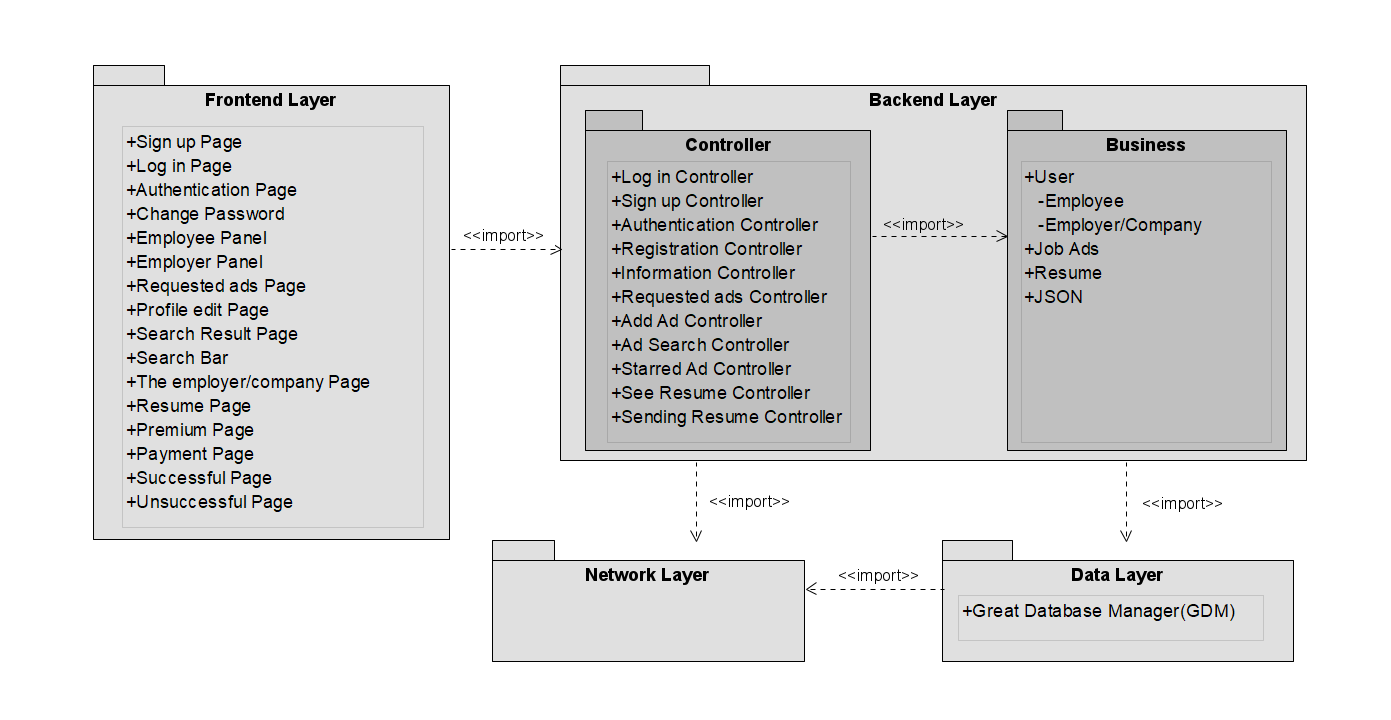
\includegraphics[width=\textwidth, height=0.5\textheight]{./images/close}
	\end{center}
	\caption{نمودار بسته‌}
	\label{pic:close-design}
\end{figure}

\section{قوانین طراحی نرم‌افزار}
بسیاری از مشکلات طراحی بر بهره‌وری و کیفیت نرم‌افزار تاثیر منفی گذاشته و هزینه‌های نگهداری نرم‌افزار را به‌شدت افزایش می‌دهند. یکی از راه‌حل‌های پیشنهاد شده برای حل اینگونه مسائل، قوانین طراحی نرم‌افزار است. استفاده‌ی صحیح آنها در طراحی نرم‌افزار، می‌تواند کیفیت نرم‌افزار را به‌شدت افزایش دهد. سامانه‌ی \textit{کارتاپ} با درنظرگرفتن این قوانین که در ادامه با جزئیات، بیان شده است، سعی کرده است که کیفیت نرم‌افزاری خود را بهبود بدهد.

\subsection{طراحی برای تغییر}
سامانه‌ی \textit{کارتاپ} به دلیل وجود یک سری رویداد، ممکن است دچار تغییراتی شود که برخی از این رویداد‌ها عبارتند از:

\begin{itemize}
	\item 
	وقوع اختلالات سیستمی و باگ‌های منجر به تغییر نیاز‌مندی‌های نرم‌افزاری
	
	\item 
	تغییر در قوانین و دستور‌العمل‌های محیط کسب‌وکار
	
	\item 
	تغییرات نرم‌افزاری سیستم بدلایل مختلف مانند بروزرسانی و بهبود امنیت سیستم
	
	\item 
	تغییرات سخت‌افزاری و ابزار‌های موردنیاز جهت پیاده‌سازی سیستم
	
	\item 
	ایجاد بهبود‌های موردنیاز‌ بنا بر بازخورد مشتری
	
	\item 
	تغییر زمان تحویل پروژه و بودجه اختصاص داده شده
\end{itemize}

مزیت \textit{کارتاپ} در چندلایه بودن معماری آن است و تا جایی که ممکن بوده سعی شده که لایه‌های معماری سیستم وابستگی بسیار کمی به یکدیگر و هر کدام از زیرسیستم‌ها استقلال داشته باشند. به این صورت که در صورت وقوع هرگونه تغییر اختمالی در زیرسیستم مورد نظر، سایر زیرسیستم‌ها تا حد امکان دست‌نخورده باقی خواهند ماند و این تغییرات به‌ آسانی صورت می‌گیرد.

\subsection{جداسازی دغدغه‌ها}
جداسازی دغدغه‌ها\RTLfootnote{\lr{Separation of Concerns} ایده‌ی مطرح شده ادسگر دایکسترا می‌باشد.}؛ این ایده بیان می‌کند که بجای تمرکز یکباره و همزمان به همه‌ی جنبه‌های یک مسئله، هر بار بر \textit{یکی} از جنبه‌ها و جدا از سایر آنها، تمرکز می‌شود که از انواع نمودار‌ها در این سند به همین سبب استفاده شده است. چسبندگی بالا در اثر پیاده‌سازی این کار در پروژه و تفکیک مسئولیت‌ها و دغدغه‌های گوناگون است. بنا بر تقسیم‌بندی وظایف، هر لایه دغدغه‌ی مربوط به خود را دارد؛ به عنوان مثال لایه‌ی واسط گرافیکی \textit{تنها} وظیفه‌ی نمایش اطلاعات را بر عهده دارد و لایه‌ی پایگاه‌داده، \textit{تنها} اطلاعات مربوط به کاربران را ذخیره و بازیابی می‌کند.

\subsection{پنهان‌سازی اطلاعات}
قانون پنهان‌سازی اطلاعات
\RTLfootnote{نخستین بار توسط دیوید پارناس به عنوان یک قانون طراحی معرفی گردید.}؛
مطابق این قانون، جزئیات پیاده‌سازی یک بدنه‌ی نرم‌افزاری، برای کاهش اثرات تغییر آن بر سایر قسمت‌های سیستم نرم‌افزاری، مخافظت می‌شود. \lr{N-Tier} بودن معماری سامانه‌ی \textit{کارتاپ} باعث شده که اطلاعات بصورت کلی قابل دسترسی و مشاهده نباشند و هر کدام از زیرسیستم‌های مستقل به اطلاعات مربوط به خود دسترسی داشته باشند و قابلیت دستیبابی به داده‌های موجود در سایر زیرسیستم‌ها وجود نداشته باشد.

\subsection{چسبندگی زیاد}
قانون چسبندگی زیاد توصیه می‌کند که طراحی پیمانه‌ها
\RTLfootnote{\lr{Modules}} باید طوری باشد که توابع هر پیمانه، بیشترین درجه‌ی ارتباط با مسئولیت اصلی پیمانه را داشته باشند. اعمال قانون چسبندگی زیاد در طراحی معماری به این معناست که مولفه‌ها و کلاس‌های هر زیرسیستم باید تا حدود زیادی به مسئولیت اصلی زیرسیستم مرتبط باشند. در سامانه‌ی \textit{کارتاپ} هدف کلی از وظایف محول شده به هر لایه، اجرا محقق شدن آرمان کل سیستم است و هر لایه‌ی معماری \textit{کارتاپ} توابع و کلاس‌های مربوط به خود را داراست.

\subsection{جفت‌شدگی کم}
استفاده از قانون جفت‌شدگی کم در طراحی معماری، به معنای کاهش اثرات زمان اجرا و تاثیر تغییر در سیستم بر زیرسیستم‌ها دیگر است. بخصوص، طراحی باید از متغیر‌های کنترلی دارای بیش از دو مقدار اجتناب نماید. بعلاوه، برای کاستن تاثیر تغییر، می‌توان از قوانین طراحی برای تغییر و پنهان‌سازی اطلاعات استفاده کرد و با توجه به معماری \lr{N-Tier} انتخاب شده، لایه‌های سیستم جفت‌شدگی کمی دارند و بصورت مستقل هر لایه کار مربوط به خود را انجام داده و خروجی را به لایه‌های بعدی منتقل می‌کند.

\subsection{ساده و احمقانه فرض کن}
قانون ساده و احمقانه فرض کن
\RTLfootnote{\lr{Keep It Simple Stupid (KISS)}}
، طراحی‌های ساده، سرراست و قابل‌فهم را توصیه می‌کند. در این نگاه، اشیا به صورت نادان در نظر گرفته می‌شوند؛ به این معنی که هر شئ تنها توانایی انجام یک کار بخصوص را دارد و روش انجام سایر کار‌ها را نمی‌داند. تقسیم‌بندی سامانه‌ی \textit{کارتاپ} این قانون را رعایت کرده، و در هر کدام از لایه‌ها بمانند لایه‌ی واسط گرافیکی و لایه‌ی کسب‌وکار برای اجرای توابع، کلاس‌ها و اشیا به ساده‌ترین شکل ممکن تعریف شده‌اند و در نتیجه می‌توان اذعان کرد که \textit{کارتاپ} دارای اشیای احمق است.

